\documentclass[12pt]{article}
\usepackage{graphicx,import}
\usepackage[svgnames]{xcolor} 
\usepackage{fancyhdr}
\usepackage{subfig}
\usepackage{hyperref}
\usepackage{enumitem}
\usepackage[many]{tcolorbox}
\usepackage{listings}
\usepackage[a4paper, total={6in, 8in} , bottom = 25mm , top = 25mm, headheight = 1.25cm , includehead,includefoot,heightrounded ]{geometry}
\usepackage{afterpage}
\usepackage{amssymb}
\usepackage{pdflscape}
\usepackage{gensymb}
\usepackage{textcomp}
\usepackage{tikz,pgfplots}
\usepackage{xecolor}
\usepackage{rotating}
\usepackage{pdfpages}
\usepackage[T1]{fontenc}
\usepackage{tikz}
\usepackage[utf8]{inputenc}
\usepackage{PTSerif} 
\usepackage{seqsplit}
\usepackage{fancyvrb}
\usepackage{mips}
\usepackage{multirow}
\usepackage{hhline}
\usepackage[edges]{forest}
\usepackage{tabularx}
\usepackage{float}
\usepackage{graphicx}
\usepackage{cprotect}
\usepackage{url}
\usepackage{listings}
\usepackage{xcolor}
\usepackage{pifont}
\newcommand{\xmark}{\ding{55}}%
\def\checkmark{\tikz\fill[scale=0.4](0,.35) -- (.25,0) -- (1,.7) -- (.25,.15) -- cycle;}

\hypersetup{
	colorlinks   = true, %Colours links instead of ugly boxes
	urlcolor     = blue, %Colour for external hyperlinks
	linkcolor    = blue, %Colour of internal links
	citecolor   = red %Colour of citations
}

\definecolor{codegreen}{rgb}{0,0.6,0}
\definecolor{codegray}{rgb}{0.5,0.5,0.5}
\definecolor{codepurple}{rgb}{0.58,0,0.82}
\definecolor{backcolour}{rgb}{0.95,0.95,0.92}
\definecolor{mGreen}{rgb}{0,0.6,0}
\definecolor{mGray}{rgb}{0.5,0.5,0.5}
\definecolor{mPurple}{rgb}{0.58,0,0.82}
\definecolor{backgroundColour}{rgb}{0.95,0.95,0.92}

\NewDocumentCommand{\codeword}{v}{
	\texttt{\textcolor{blue}{#1}}
}
\lstset{language=java,keywordstyle={\bfseries \color{blue}}}
\definecolor{dkgreen}{rgb}{0,0.6,0}
\definecolor{gray}{rgb}{0.5,0.5,0.5}
\definecolor{mauve}{rgb}{0.58,0,0.82}



\lstdefinestyle{mystyle}{
	backgroundcolor=\color{backcolour},   
	commentstyle=\color{codegreen},
	keywordstyle=\color{magenta},
	numberstyle=\tiny\color{codegray},
	stringstyle=\color{codepurple},
	basicstyle=\ttfamily\normalsize,
	breakatwhitespace=false,         
	breaklines=true,                 
	captionpos=b,                    
	keepspaces=true,                 
	numbers=left,                    
	numbersep=5pt,                  
	showspaces=false,                
	showstringspaces=false,
	showtabs=false,                  
	tabsize=2
}

\lstdefinestyle{CStyle}{
	backgroundcolor=\color{backgroundColour},   
	commentstyle=\color{mGreen},
	keywordstyle=\color{magenta},
	numberstyle=\tiny\color{mGray},
	stringstyle=\color{mPurple},
	basicstyle=\footnotesize,
	breakatwhitespace=false,         
	breaklines=true,                 
	captionpos=b,                    
	keepspaces=true,                 
	numbers=left,                    
	numbersep=5pt,                  
	showspaces=false,                
	showstringspaces=false,
	showtabs=false,                  
	tabsize=2,
	language=C
}



\lstset{ %
	language=[mips]Assembler,       % the language of the code
	basicstyle=\footnotesize,       % the size of the fonts that are used for the code
	numbers=left,                   % where to put the line-numbers
	numberstyle=\tiny\color{gray},  % the style that is used for the line-numbers
	stepnumber=1,                   % the step between two line-numbers. If it's 1, each line
	% will be numbered
	numbersep=5pt,                  % how far the line-numbers are from the code
	backgroundcolor=\color{white},  % choose the background color. You must add \usepackage{color}
	showspaces=false,               % show spaces adding particular underscores
	showstringspaces=false,         % underline spaces within strings
	showtabs=false,                 % show tabs within strings adding particular underscores
	frame=single,                   % adds a frame around the code
	rulecolor=\color{black},        % if not set, the frame-color may be changed on line-breaks within not-black text (e.g. commens (green here))
	tabsize=4,                      % sets default tabsize to 2 spaces
	breaklines=true,                % sets automatic line breaking
	breakatwhitespace=false,        % sets if automatic breaks should only happen at whitespace
	% also try caption instead of title
	keywordstyle=\color{blue},          % keyword style
	commentstyle=\color{dkgreen},       % comment style
	stringstyle=\color{mauve},         % string literal style
	escapeinside={\%*}{*)},            % if you want to add a comment within your code
	morekeywords={*,...}               % if you want to add more keywords to the set
}

\setmainfont[ExternalLocation=fonts/]{EBGaramond-Regular.ttf}


\newenvironment{changemargin}[2]{%
	\begin{list}{}{%
			\setlength{\topsep}{0pt}%
			\setlength{\leftmargin}{#1}%
			\setlength{\rightmargin}{#2}%
			\setlength{\listparindent}{\parindent}%
			\setlength{\itemindent}{\parindent}%
			\setlength{\parsep}{\parskip}%
		}%
		\item[]}{\end{list}}


\definecolor{foldercolor}{RGB}{124,166,198}

\tikzset{pics/folder/.style={code={%
			\node[inner sep=0pt, minimum size=#1](-foldericon){};
			\node[folder style, inner sep=0pt, minimum width=0.3*#1, minimum height=0.6*#1, above right, xshift=0.05*#1] at (-foldericon.west){};
			\node[folder style, inner sep=0pt, minimum size=#1] at (-foldericon.center){};}
	},
	pics/folder/.default={20pt},
	folder style/.style={draw=foldercolor!80!black,top color=foldercolor!40,bottom color=foldercolor}
}

\forestset{is file/.style={edge path'/.expanded={%
			([xshift=\forestregister{folder indent}]!u.parent anchor) |- (.child anchor)},
		inner sep=1pt},
	this folder size/.style={edge path'/.expanded={%
			([xshift=\forestregister{folder indent}]!u.parent anchor) |- (.child anchor) pic[solid]{folder=#1}}, inner xsep=0.6*#1},
	folder tree indent/.style={before computing xy={l=#1}},
	folder icons/.style={folder, this folder size=#1, folder tree indent=3*#1},
	folder icons/.default={12pt},
}

\begin{document}
	
	
	%%% title pages
	\begin{titlepage}
		\begin{center}
			
			\vspace*{0.7cm}
			
			
\includegraphics[width=0.4\textwidth]{sharif1.png}\\
			\vspace{0.5cm}
			\textbf{ \Huge{Multicore Computing} }\\
			\vspace{0.5cm}
			\textbf{ \Large{ Project - Edge Detection Filter} }
			\vspace{0.2cm}
			
			
			\large \textbf{Department of Computer Engineering}\\\vspace{0.2cm}
			\large   Sharif University of Technology\\\vspace{0.2cm}
			\large   Spring 2022 \\\vspace{0.2cm}
			\noindent\rule[1ex]{\linewidth}{1pt}
			Lecturer:\\
			\textbf{{Dr. Falahati}}
			
			
			\vspace{0.15cm}
			Name - Student Number:\\
			
			\textbf{{Saba Hashemi - 97100581}}\\
			
			\textbf{{Amirmahdi Namjoo - 97107212}}
		\end{center}
	\end{titlepage}
	%%% title pages
	
	
	%%% header of pages
	\newpage
	\pagestyle{fancy}
	\fancyhf{}
	\fancyfoot{}
	\cfoot{\thepage}
	\chead{ Amirmahdi Namjoo - Saba Hashemi}
	\rhead{
\includegraphics[width=0.1\textwidth]{sharif.png}}
	\lhead{Project}
	%%% header of pages
	
	
	
		\section{Team Members}
	
	\begin{itemize}
		
		\item Team member No.1: Saba Hashemi, 97100581
		\item Team member No.2: Amirmahdi Namjoo, 97107212
	\end{itemize}
	
\newpage
	\section{Introduction}
	
	
In this project, we implemented an Edge Detection Filter based on Sobel Filter. The project's core is based on SIMD computations using NVIDIA CUDA. The project features both CLI and GUI. The GUI is written in Python, uses the Tkinter library, and communicates with the CUDA core, which is written in C++ using a shell.
\newpage

\section{Implementation}

Our project has two main parts. One part is adjusting the contrast and brightness of pictures, and the other part is Sobel Filter.

\subsection{Contrast and Brightness}

Each pixel's contrast and brightness in an image can be changed using the following formula:

$$\alpha \times \text{pixel} + \beta$$

In which $\alpha$ is contrast and $\beta$ is brightness. This formula needs to be applied to the whole image to change the contrast and brightness of an image. Due to the parallel nature of the task, it could be easily achieved using CUDA. Our Kernel for this task is as follows:

\begin{lstlisting}[language=c++]
__global__
void adjust(uchar *input,
	uchar *output,
	float alpha,
	float beta,
	size_t size) {
		/* Calculate the index of the pixel that this 
		thread is responsible for */
		int idx = blockDim.x * blockIdx.x + threadIdx.x;
		
		/* Calculate new value of the pixel*/
		uchar pixel = input[idx];
		int value = alpha * pixel + beta;

		/* Clip value to valid range */
		if (value > 255)
			value = 255;
		if (value < 0)
			value = 0;
						
		/* Store result */
		output[idx] = (uchar) value;
	}
\end{lstlisting}


\newpage


\subsection{Sobel Filter}
There exist multiple filters to implement edge detection. For this project, we used Sobel Filter. To use Sobel Filter, the whole image $\mathbf{A}$ is convolved with two matrices $\mathbf{G_x}$ and $\mathbf{G_y}$, which are shown below:

\begin{table}[ht!]
	\centering
	\begin{tabular}{|c|c|c|}
		\hline
		+1 & 0 & -1 \\ \hline
		+2 & 0 &  -2 \\ \hline
		+1 & 0 & -1 \\ \hline
	\end{tabular}
	\cprotect\caption{$\mathbf{G_x}$}
\end{table}

\begin{table}[ht!]
	\centering
	\begin{tabular}{|c|c|c|}
		\hline
		+1 & +2 & +1 \\ \hline
		0 & 0 &  0 \\ \hline
		-1 & -2 & -1 \\ \hline
	\end{tabular}
	\cprotect\caption{$\mathbf{G_y}$}
\end{table}

Then, the gradient magnitude matrix is constructed by calculating the $\sqrt{g^2_x + g^2_y}$ for all elements of $\mathbf{G_x}$ and $\mathbf{G_y}$. The resulting matrix $G = \sqrt{G^2_x + G^2_y}$ is used to show edges of the picture.

The kernel code for this part is as follows:

\begin{lstlisting}[language=c++]
__global__
void conv(uchar *input,
	uchar *output,
	float *kernel_v,
	float *kernel_h,
	size_t rows,
	size_t cols,
	size_t kernel_size) {
	/* Calculate the index of the pixel that this 
	thread is responsible for */
	int idx = blockDim.x * blockIdx.x + threadIdx.x;
	int i = idx / cols;
	int j = idx % cols;
	
	float sum_v = 0, sum_h = 0;
	/* Range over kernel entries */
	for (int kidx = 0; kidx < kernel_size * kernel_size; kidx++) {
		int ki = kidx / kernel_size;
		int kj = kidx % kernel_size;
		
		int new_i = i + ki - kernel_size / 2;
		int new_j = j + kj - kernel_size / 2;
		
		/* Pass pixel if we are out of boundry */
		if (new_i < 0 || new_i >= rows || new_j < 0 || new_j >= cols)
			continue;
		
		int new_idx = new_i * cols + new_j;

		/* Convolve each of horizontal and vertical filters
		with image */		
		sum_v += kernel_v[kidx] * (float) input[new_idx];
		sum_h += kernel_h[kidx] * (float) input[new_idx];
	}
	
	/* Calculate new value of the pixel */
	int value = (int) sqrt(sum_v * sum_v + sum_h * sum_h);

	/* Clip value to valid range */
	if (value > 255)
	value = 255;
	if (value < 0)
	value = 0;
	
	/* Store result */
	output[idx] = (uchar) value;
}
\end{lstlisting}


\subsection{Memory Management}

When calling CUDA functions, we need to ensure all arguments are stored in CUDA-accessible memory. For this reason, we used \verb+cudaMalloc+ function to allocate GPU memory and \verb+cudaMemcpy+ to copy data from host memory to device and visa-versa. Also, \verb+cudaFree+ is used to free GPU memory.

An example from the code is shown below:

\begin{lstlisting}[language=c++]
/* Allocate GPU memory for input and ouput image */
cudaMalloc(&input_image_device, total_size_bytes);
cudaMalloc(&output_image_device, total_size_bytes);

/* Copy input image to GPU memory */
cudaMemcpy(input_image_device, input_image_host, total_size_bytes, cudaMemcpyHostToDevice);

/* Do some work ... */

/* Copy output image to host memory */
cudaMemcpy(output_image_host, output_image_device, total_size_bytes, cudaMemcpyDeviceToHost);

/* Free allocated memory */
cudaFree(output_image_device);
cudaFree(input_image_device);
\end{lstlisting}

\newpage 
\section{Results}

To compare the speedup from switching to GPU, we tested five different images (included in \Verb+benchmark+ folder in \Verb+core+). The dimensions of these five images are \Verb+1920x1080+ (Full HD), \Verb+1920x1200+, \Verb+1920x1440+, \Verb+3840x2160+ (4K), \Verb+7680x4320+ (8K). As our code includes two parts, namely "Brightness and Contrast Adjustment" and "Sobel Edge Filter," we recorded the timing details of each of these parts separately. We plotted different graphs for each part and the total time of running these parts. Note that the time needed to load the picture using OpenCV and write it to the file is not included in the data.

For the GPU implementation part, we measured time for three different block sizes, "256", "64", and "16".

It is noteworthy that because the runtime of CPU implementation is orders of magnitude higher than GPU code, we plotted two different plots for each part; one includes CPU timings, and the other just includes GPU timing have better resolution.

Also, the values for Brightness and Contrast adjustment in all runs are $\alpha = 0.8, \beta=50$.

You can view the results in the charts below:

\begin{figure}[H]
	\centering
	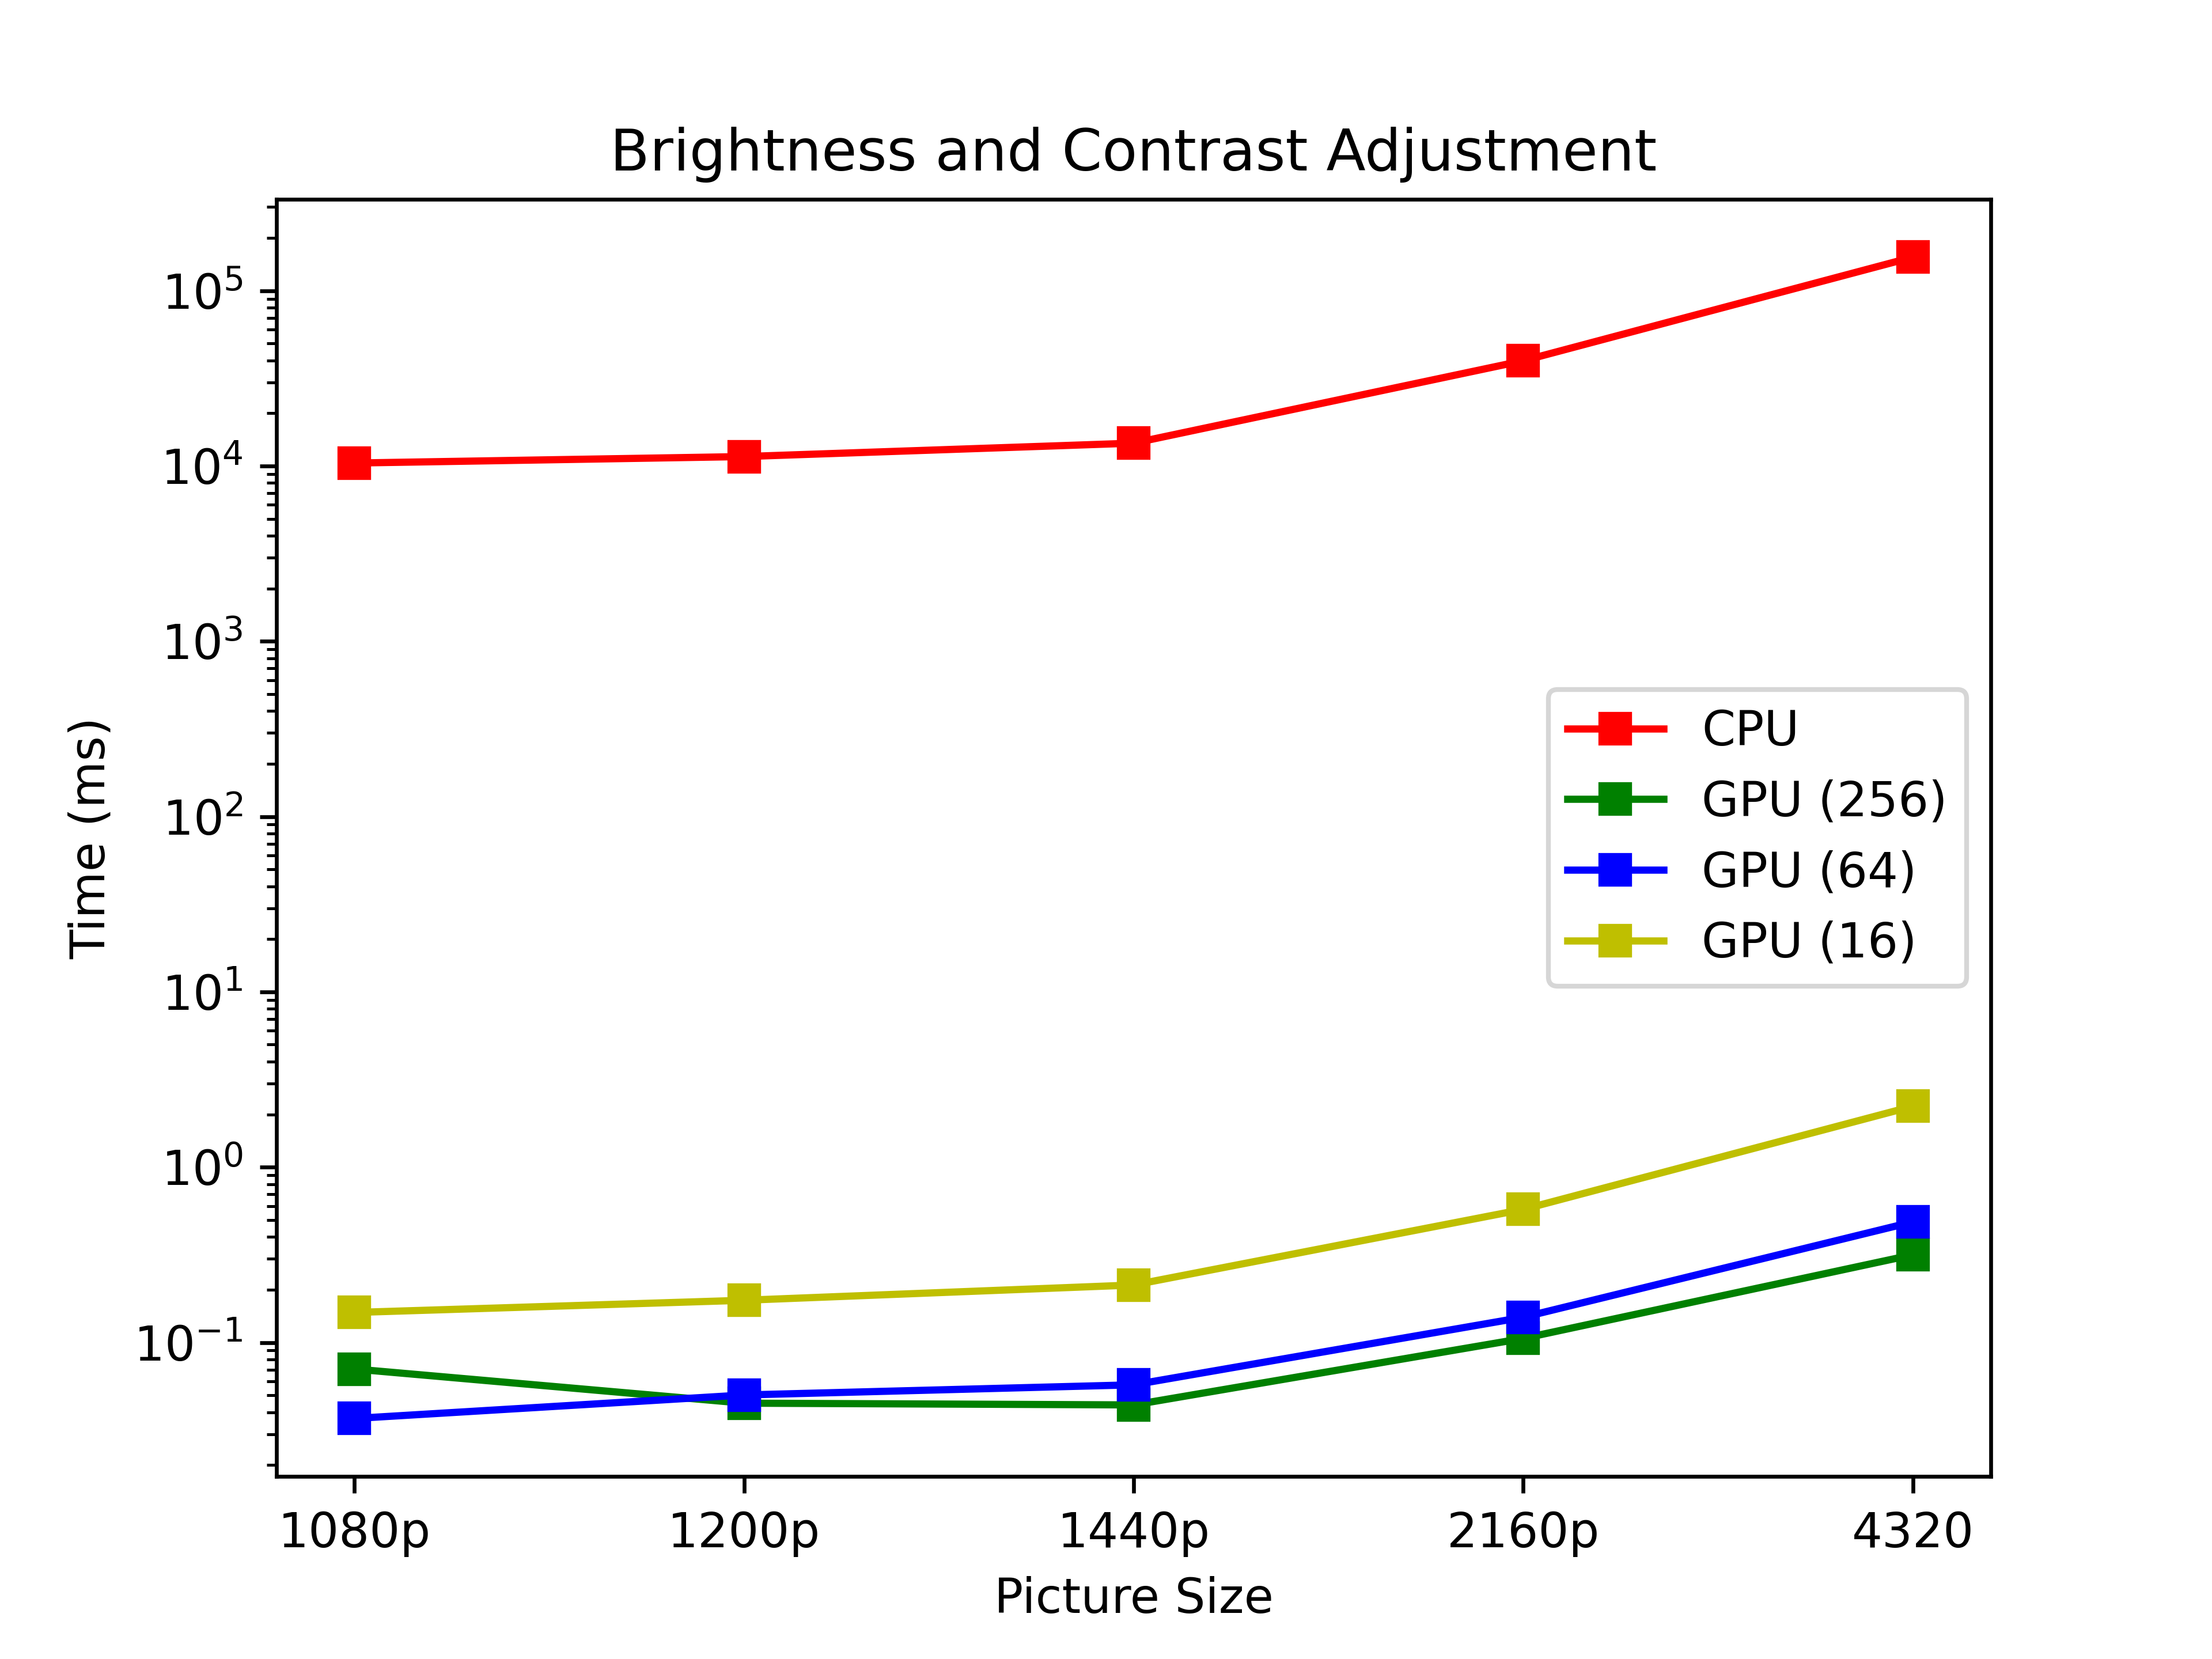
\includegraphics[width=0.8\textwidth]{./images/BCA.png}	
	\cprotect\caption{Brightness and Contrast Adjustment Benchmark (Including CPU)}
	\label{fig:1}
\end{figure}



\begin{figure}[H]
	\centering
	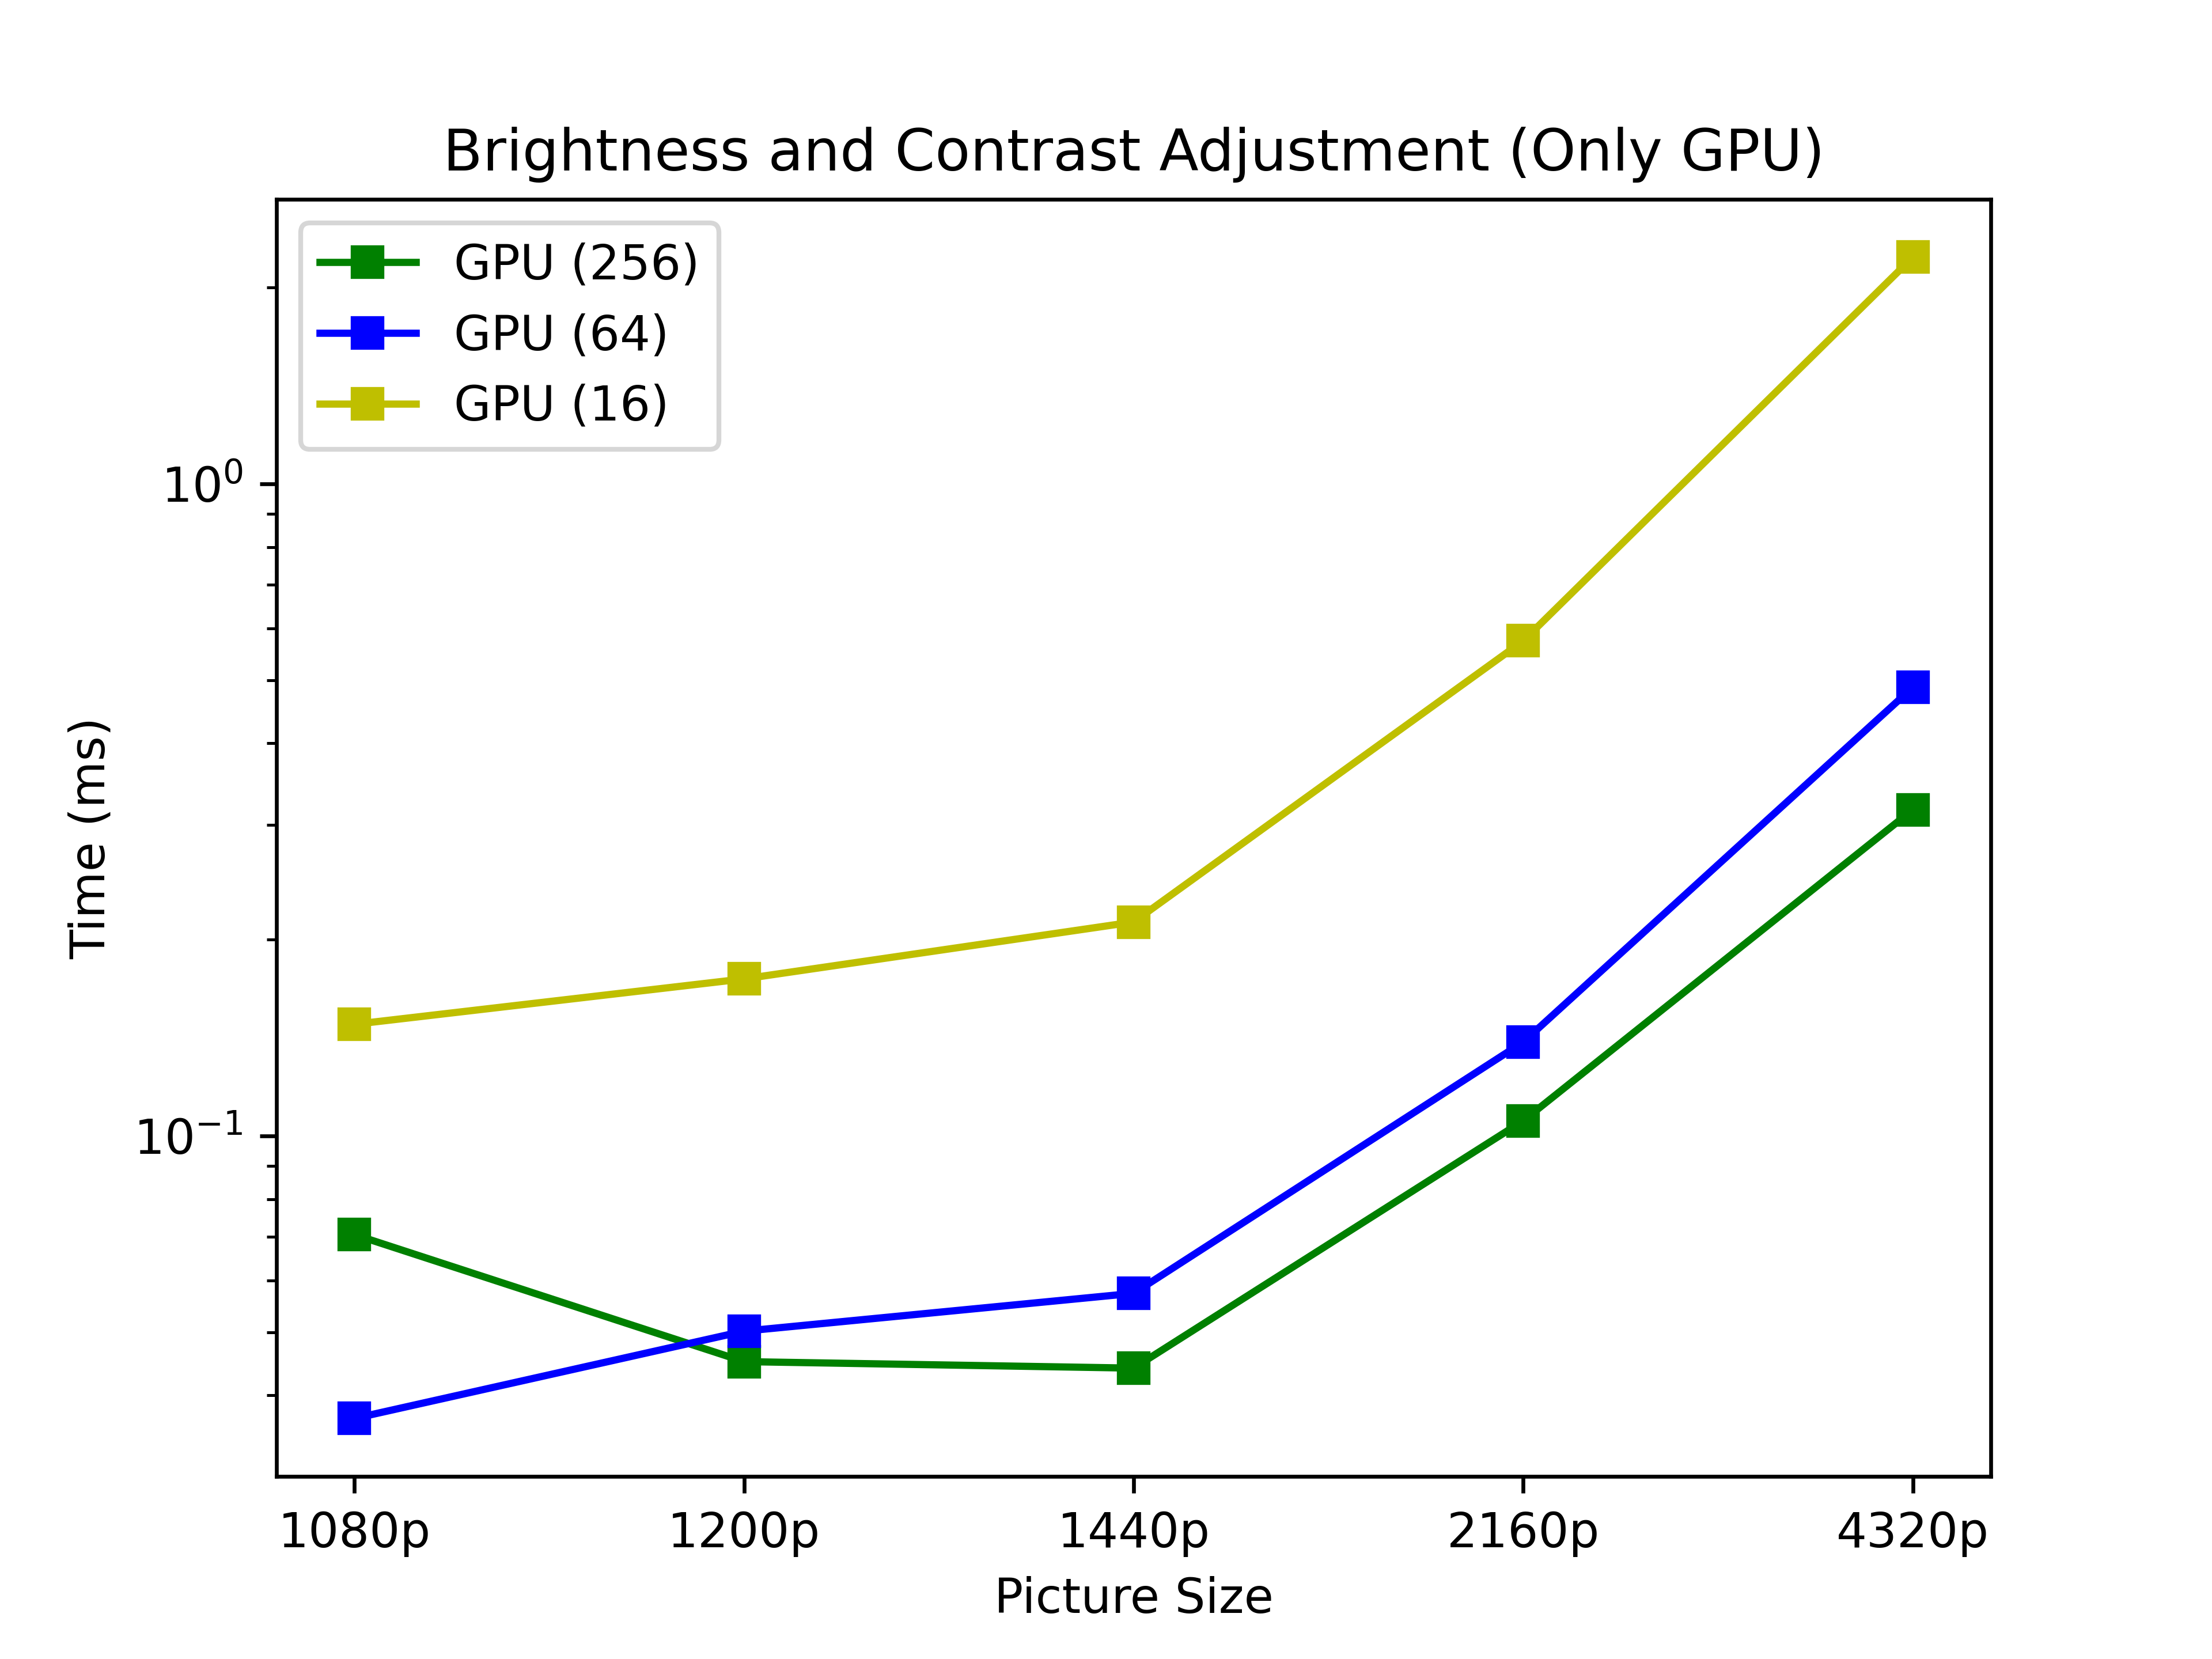
\includegraphics[width=0.8\textwidth]{./images/BCA2.png}	
	\cprotect\caption{Brightness and Contrast Adjustment Benchmark (Without CPU)}
	\label{fig:2}
\end{figure}



\begin{figure}[H]
	\centering
	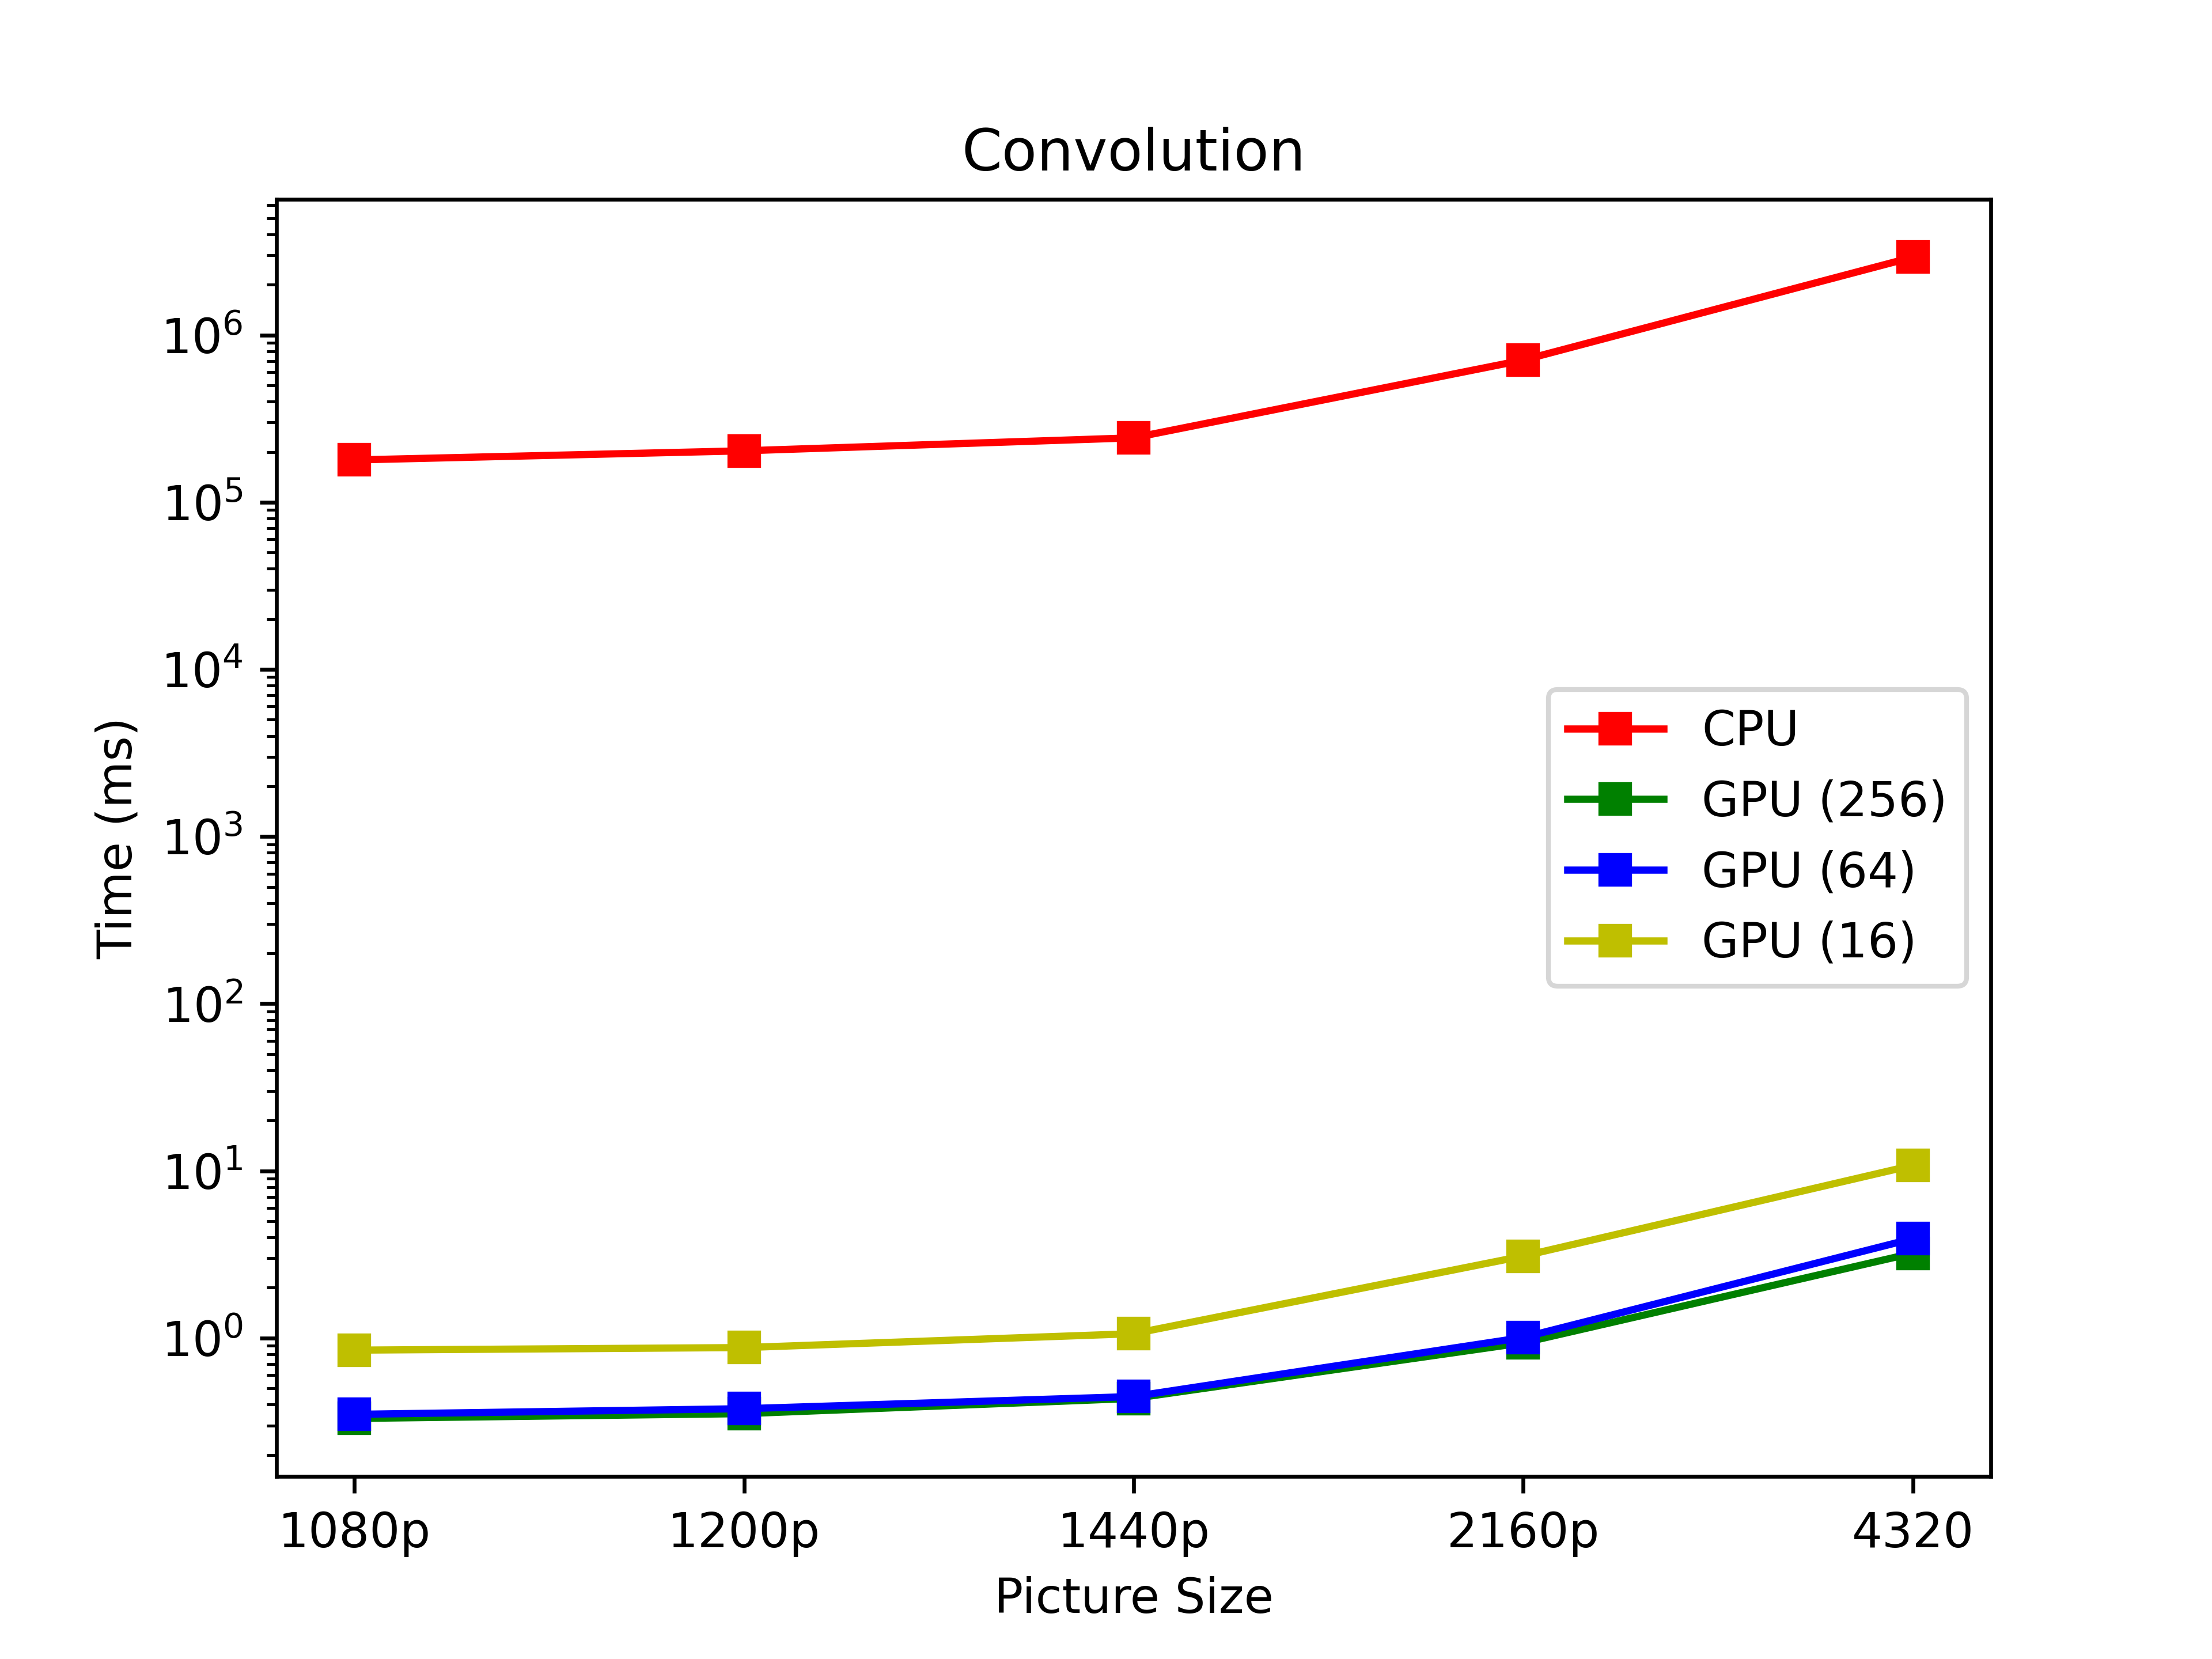
\includegraphics[width=0.8\textwidth]{./images/Convolution.png}	
	\cprotect\caption{Sobel Edge Detection Filter Convolution Benchmark  (Including CPU)}
	\label{fig:3}
\end{figure}


\begin{figure}[H]
	\centering
	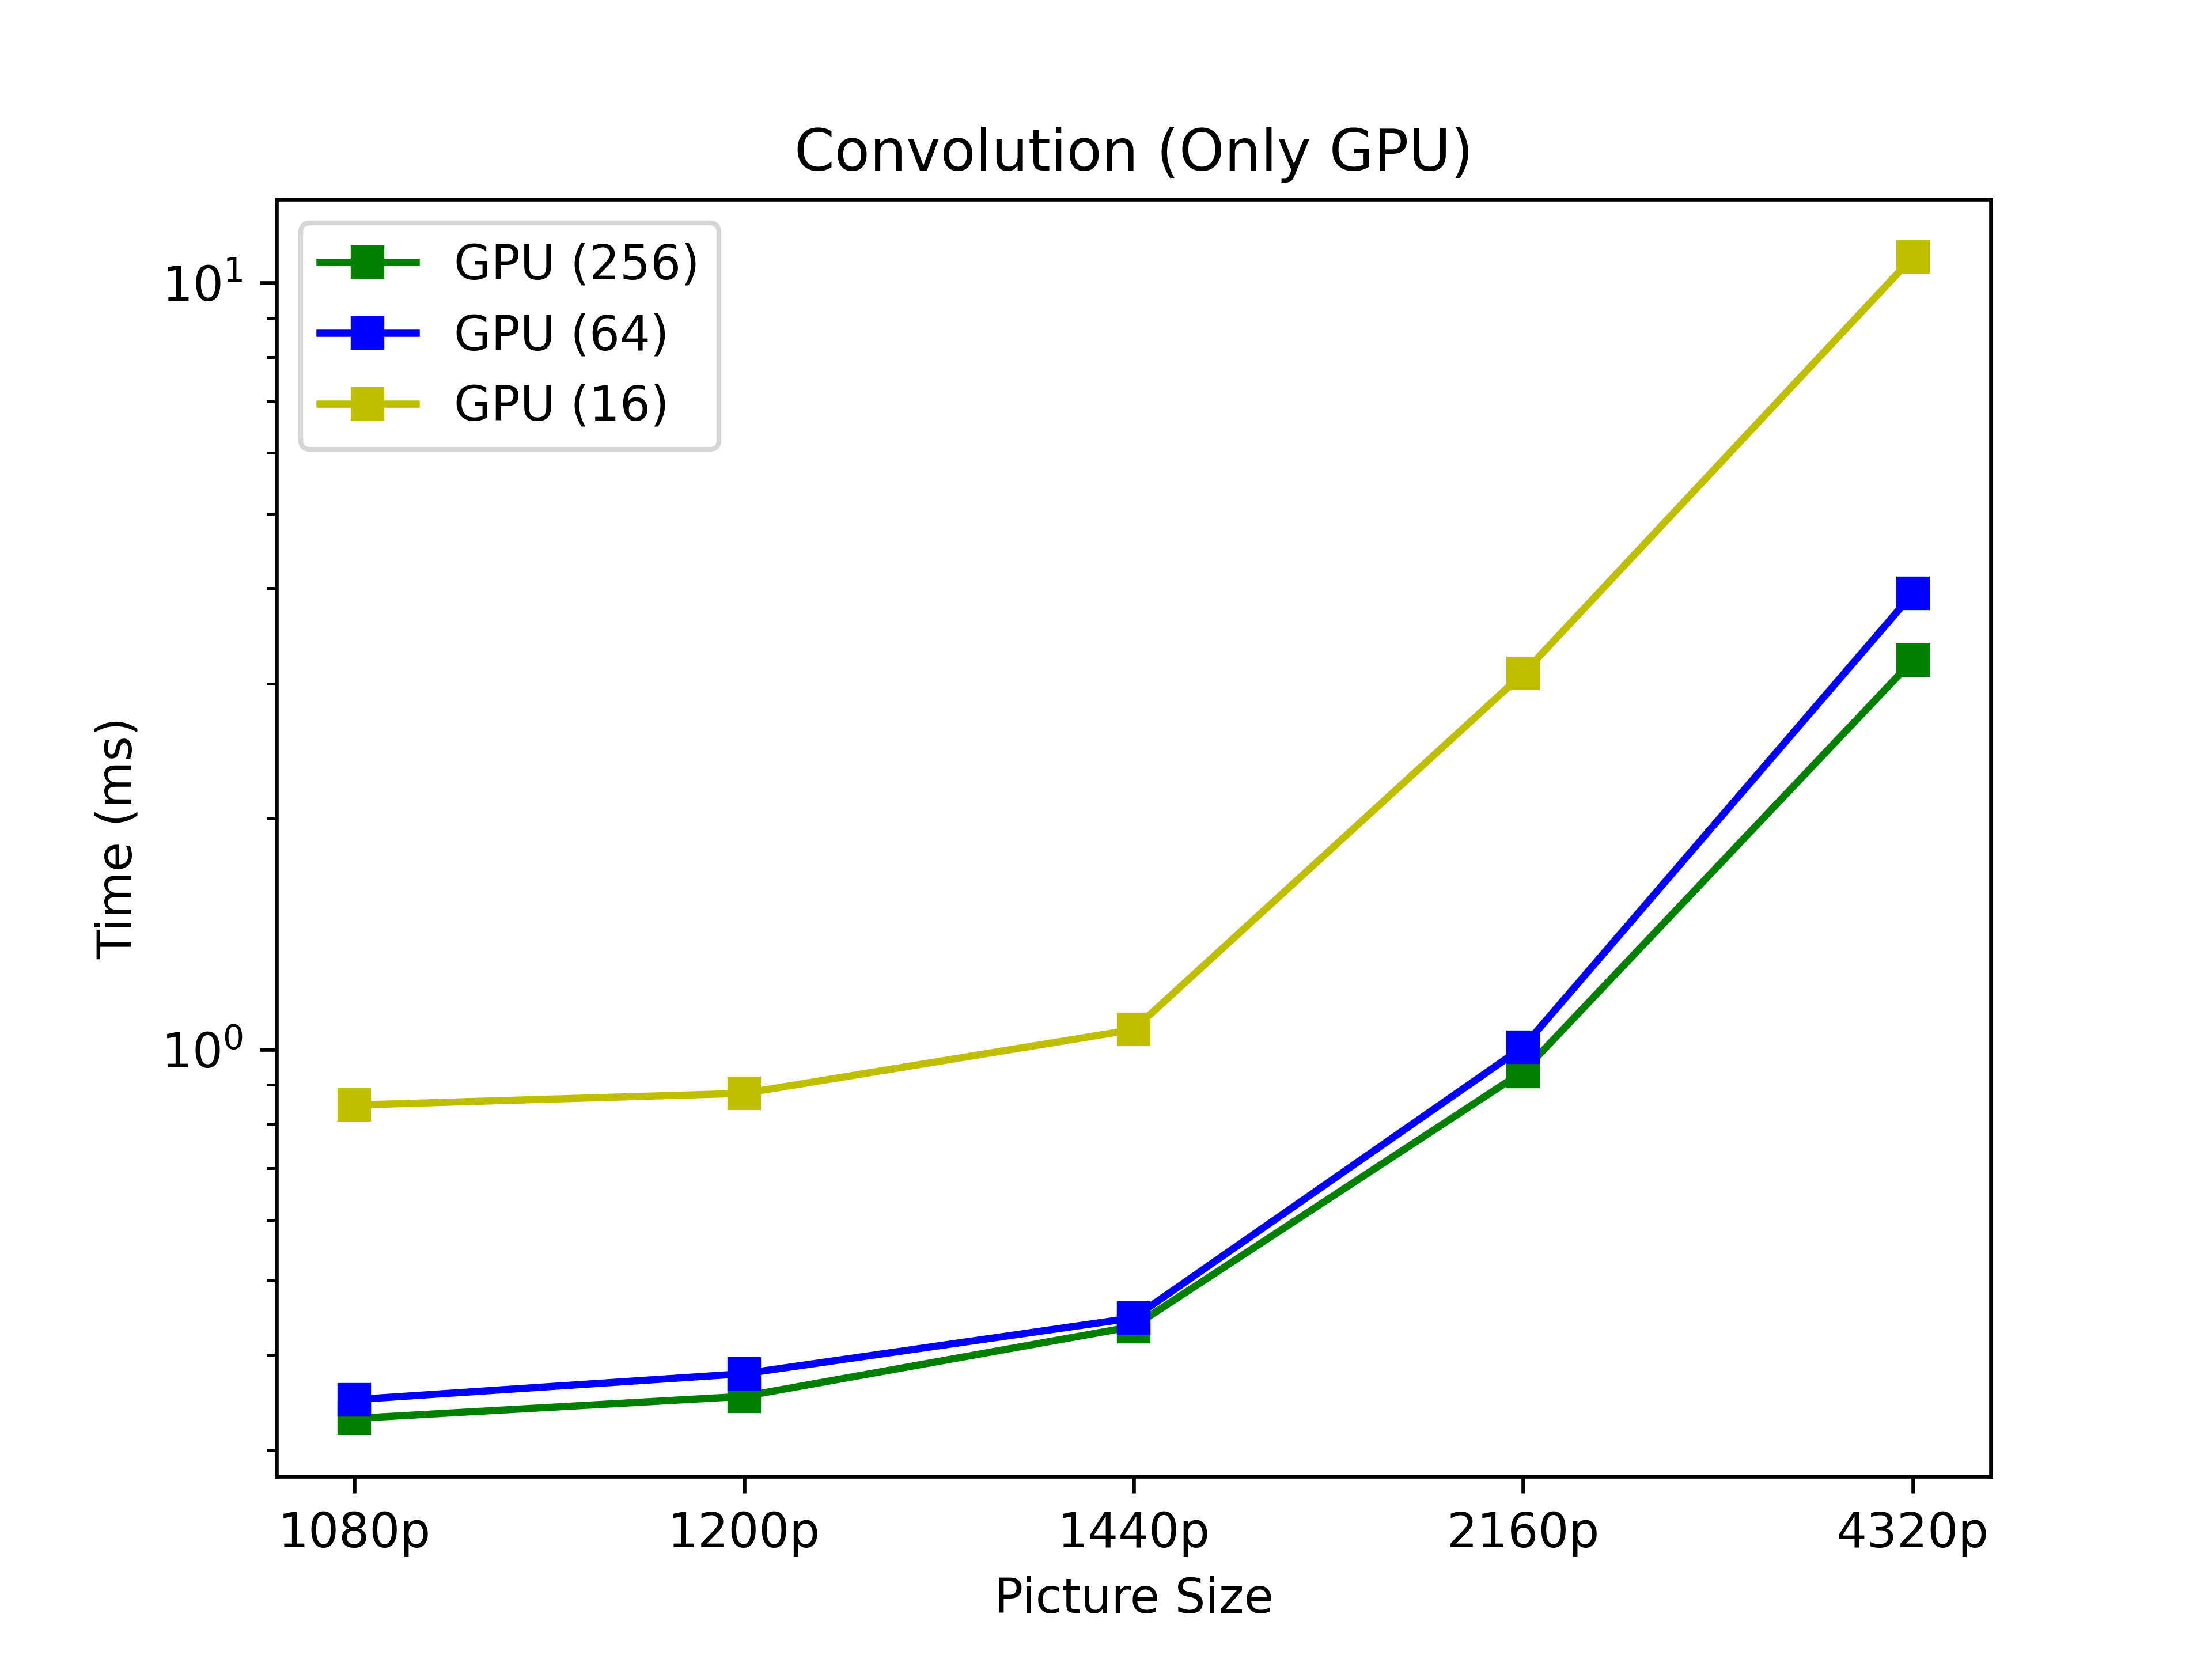
\includegraphics[width=0.8\textwidth]{./images/Convolution2.png}	
	\cprotect\caption{Sobel Edge Detection Filter Convolution Benchmark  (Without CPU)}
	\label{fig:4}
\end{figure}


\begin{figure}[H]
	\centering
	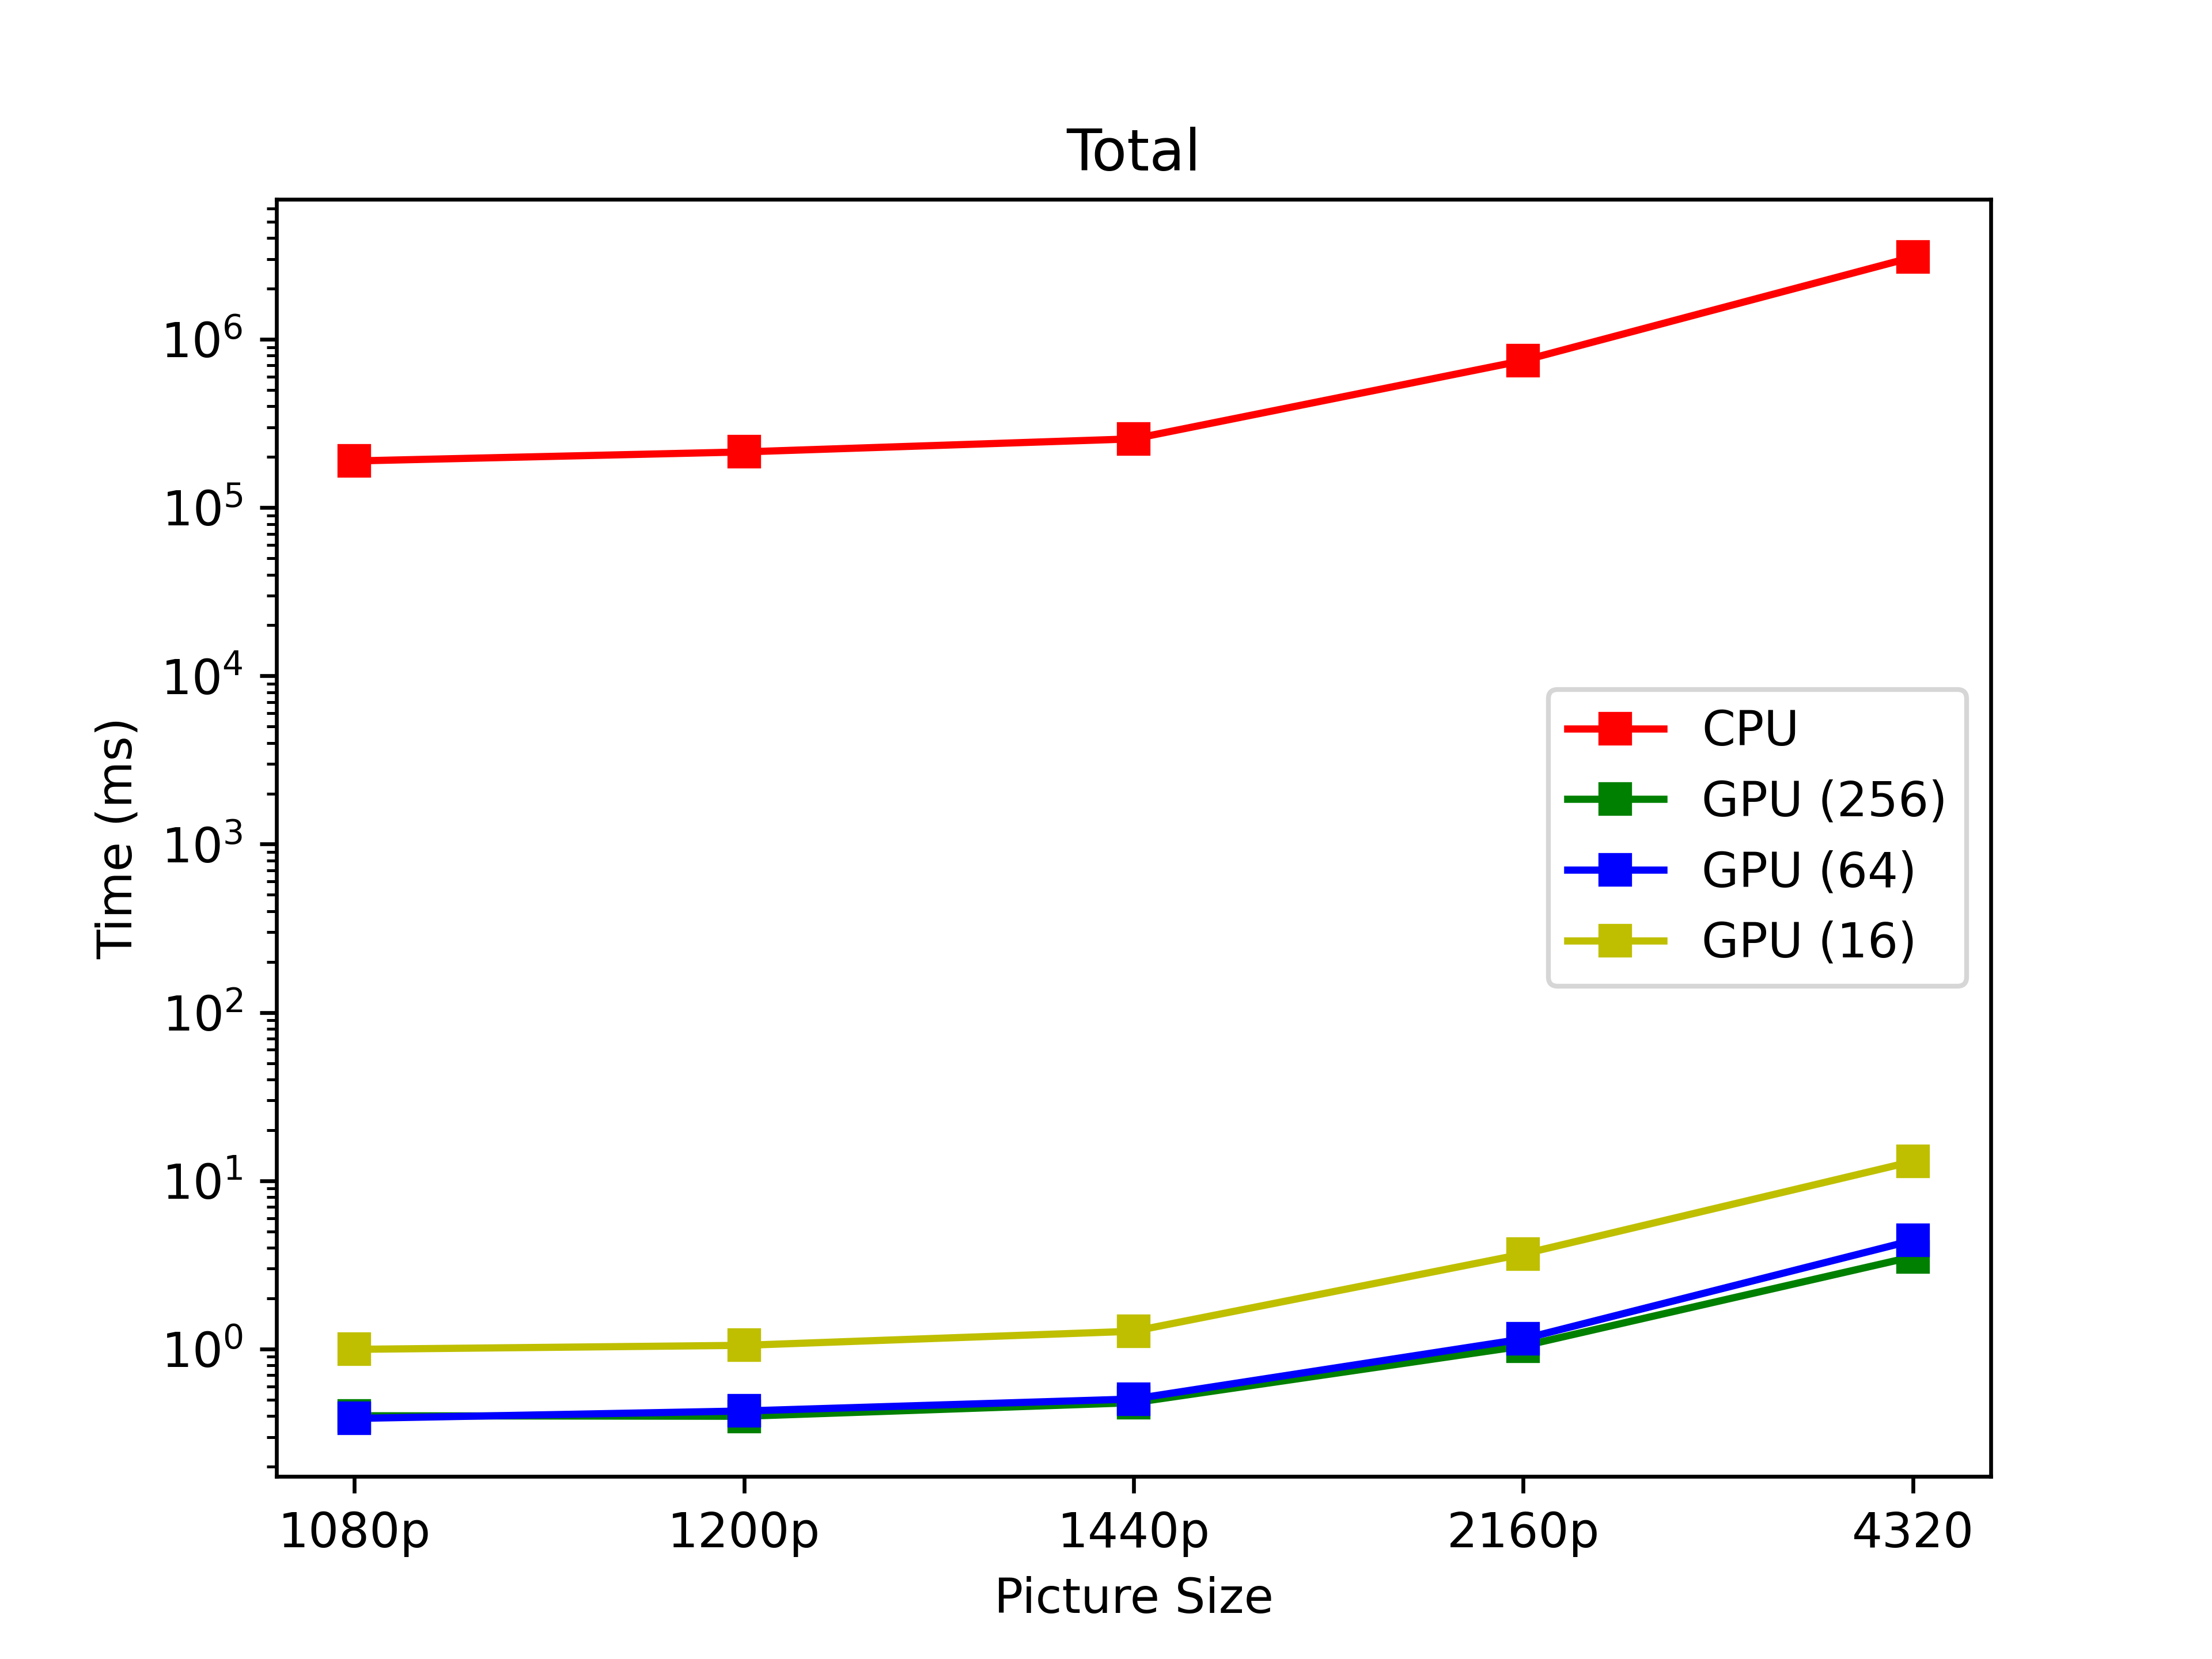
\includegraphics[width=0.8\textwidth]{./images/Total.png}	
	\cprotect\caption{Total Runtime Benchmark  (Including CPU)}
	\label{fig:5}
\end{figure}



\begin{figure}[H]
	\centering
	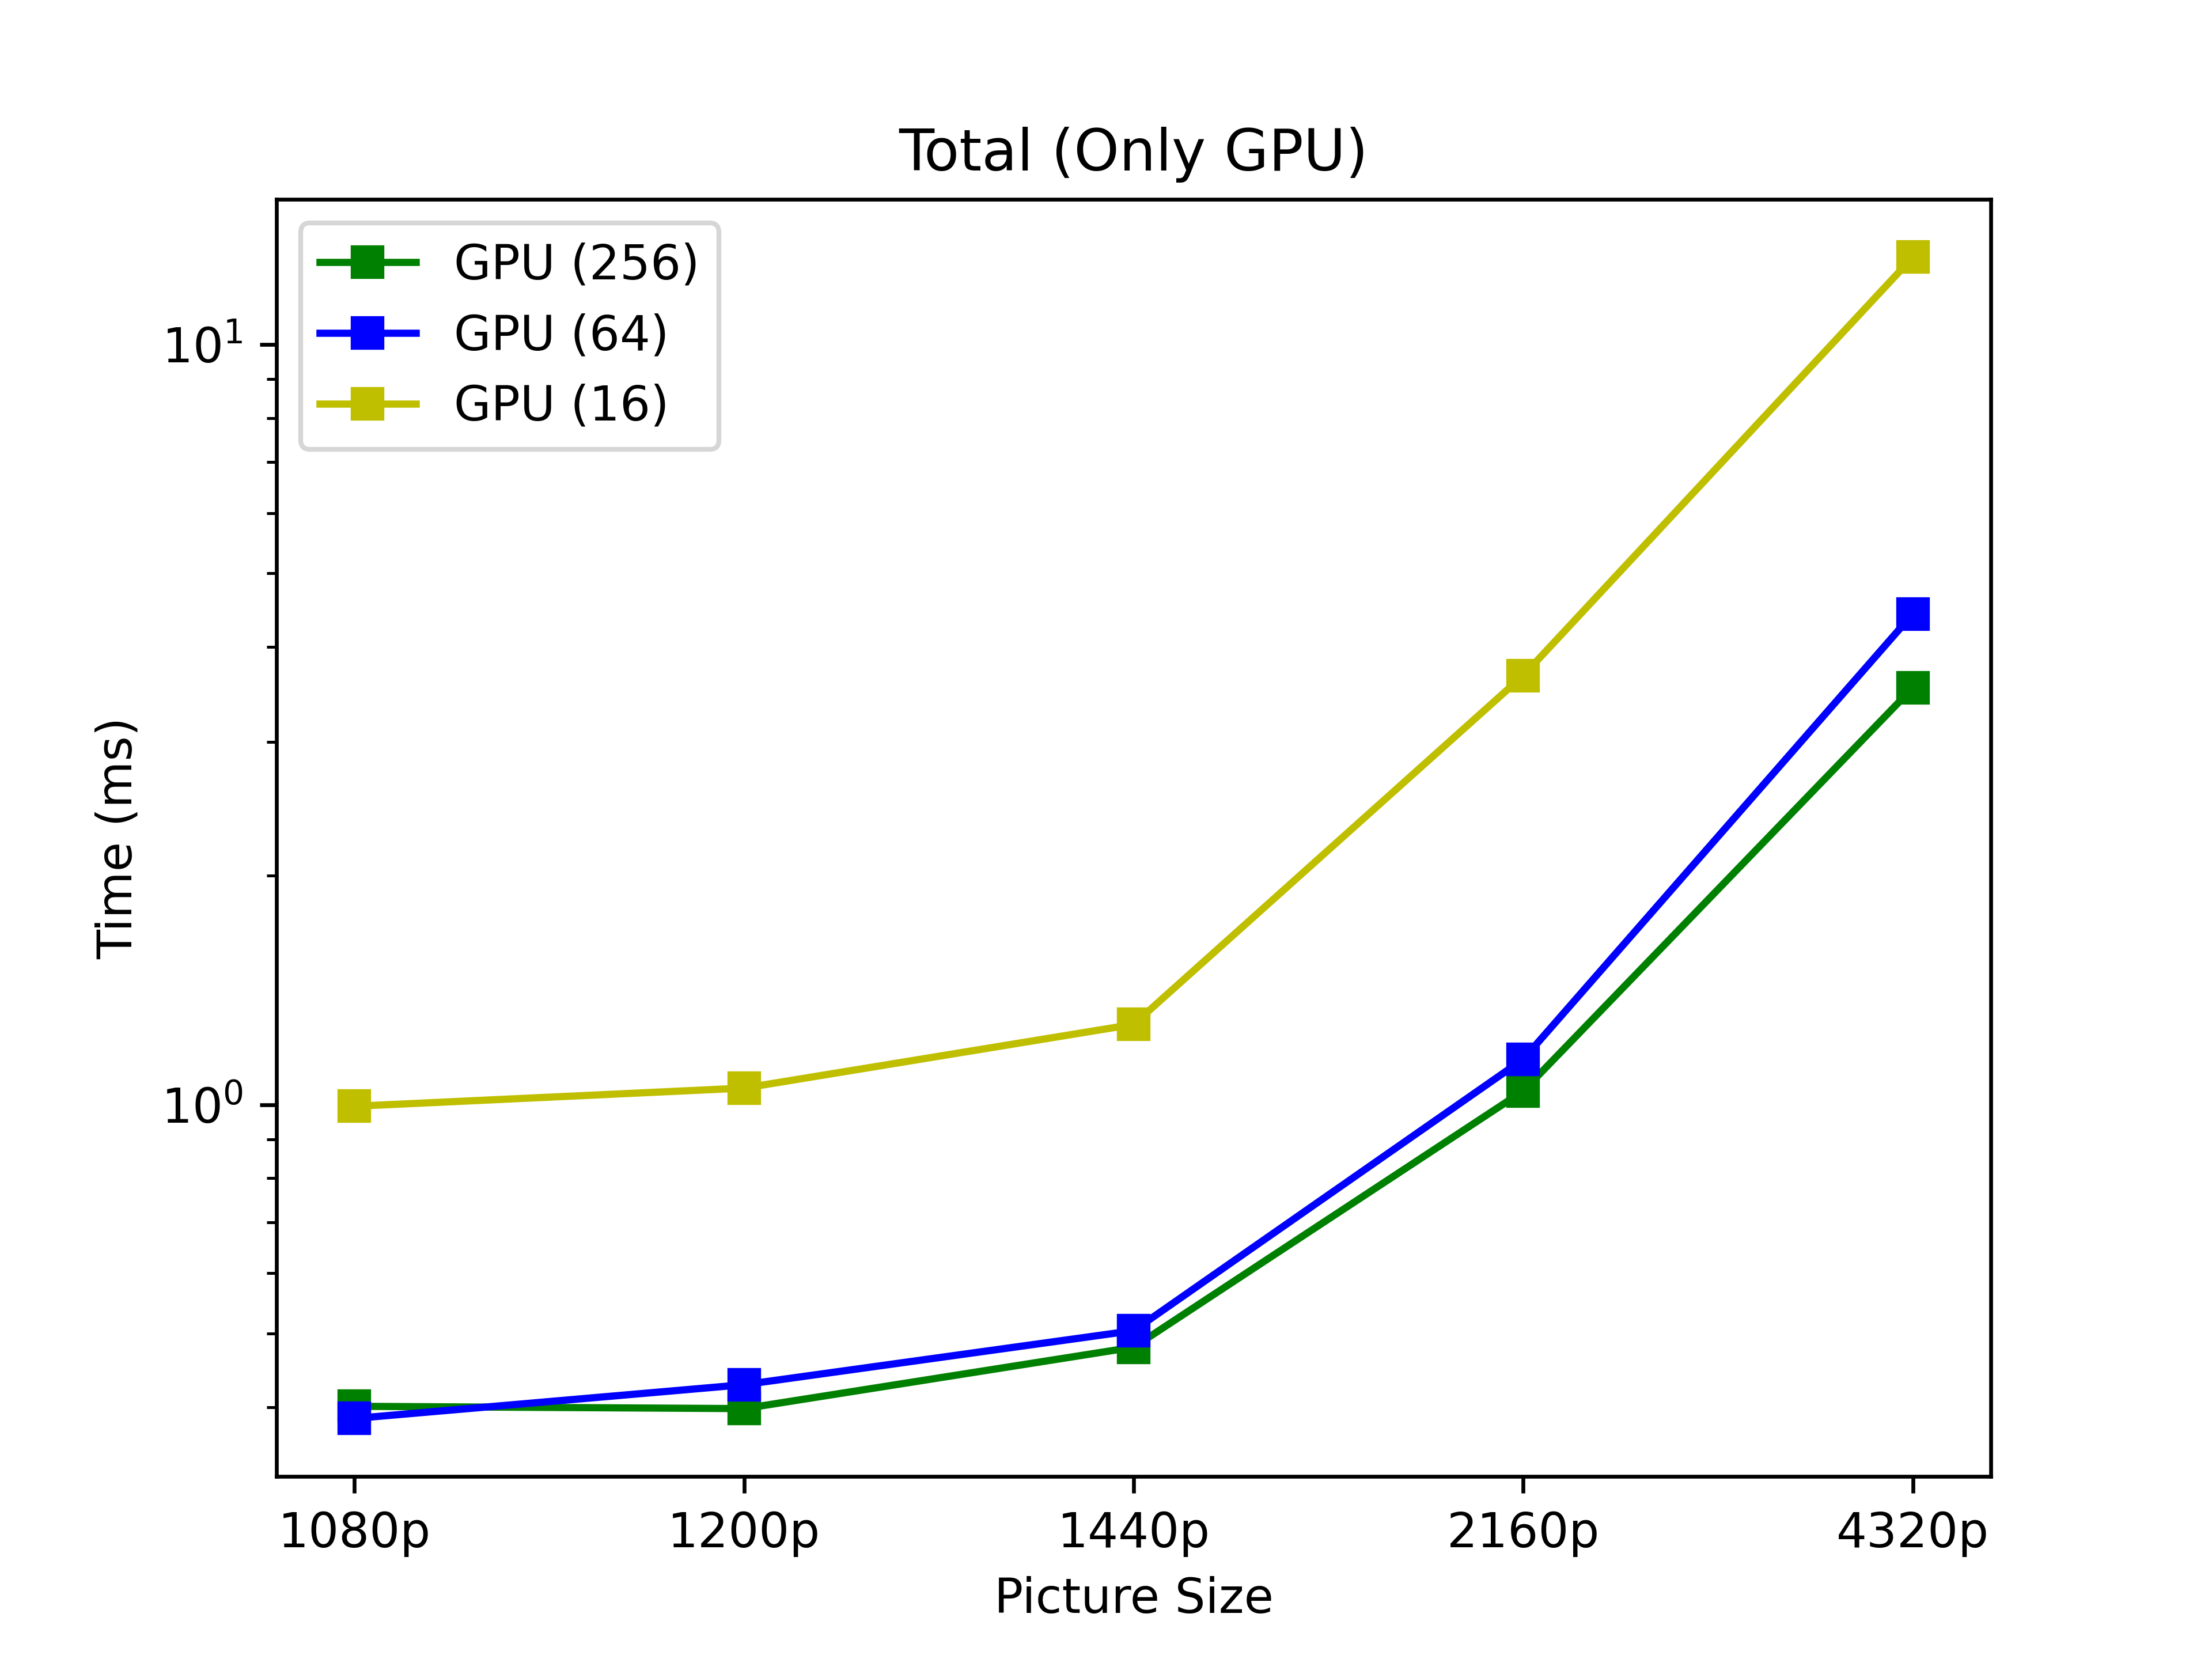
\includegraphics[width=0.8\textwidth]{./images/Total2.png}	
	\cprotect\caption{Total Runtime Benchmark  (Without CPU)}
	\label{fig:6}
\end{figure}

As evident from the plots, we gain a huge exponential speedup by using GPU and CUDA. Also, in most cases, "256 threads per block" was the best option. While, in most cases, the difference between 256 and 64 is minor, the difference between 16 and 256 is substantial.



\end{document}
